\subsection{Linearization of the plant}

Multiple sources indicate, that linearization needs to be considered. “PID is a linear-type controller and hence is only efficient for a limited operating range when used to control non-linear processes.” \cite{PIDLinear1} “PID controllers perform well only on linear systems or systems that are linearized.” \cite{PIDLinear2} “PID control can only be applied for linear plant dynamics 99 percent of applications” \cite{PIDLinear3} 

As the quadcopter, is a non-linear system, due to its non-linear terms in the plant equations, to use PID, linearization would be needed. It is planned to have three PID controllers: Z, $\phi$/roll, and $\theta$/pitch. The equations below indicate that the only non-linear equation is Z.
\begin{displaymath}
    \ddot{\phi} = \frac{\dot{\theta}\dot{\psi}(I_{yy}-I_{zz})-J_r\dot{\theta}\omega_r+l(U_2)}{I_{xx}}
\end{displaymath}
\begin{displaymath}
    \ddot{\theta} = \frac{\dot{\phi}\dot{\psi}(I_{zz}-I_{xx})-J_r\dot{\phi}\omega_r+l(U_3)}{I_{yy}}
\end{displaymath}
\begin{displaymath}
    \ddot{Z} = \frac{mg - (cos\theta cos \phi )U_1 - A_z\dot{Z} }{m}
\end{displaymath}
The non-linear terms are due to $\phi$ and $\theta$. There is a simple way of linearizing the Z-axis plant equation, as the intended goal is only hovering. 
For hovering, $\phi$, and $\theta$ would be zero, which would be ensured due to PID control to respective axis, they would become constants, thus the non-linear terms 
\begin{displaymath}
    cos(\phi)*cos(\theta) \longrightarrow cos(0)*cos(0) = 1
\end{displaymath}
\begin{displaymath}
    \ddot{Z} = \frac{mg - (cos\theta cos \phi )U_1 - A_z\dot{Z} }{m} \longrightarrow \ddot{Z} = \frac{mg - U_1 - A_z\dot{Z} }{m}
\end{displaymath}

Thus the plant Z-axis equation is linearized. Only downside, is to accept this assumtion, it should be ensured, that $\phi$ and $\theta$ PID controllers should be calibrated first, to ensure, that the values remain zero, when calibrating Z-axis PID.

The motors need to be linearized to work with the PID. It is known from testing that the motors can output a maximum angular speed of 3500 at 255 PWM. To convert from PWM to angular speed, we divide the two with PWM as the numerator. Below is a graph that shows the linear graph of this.

\begin{figure}[H]
\begin{center}
   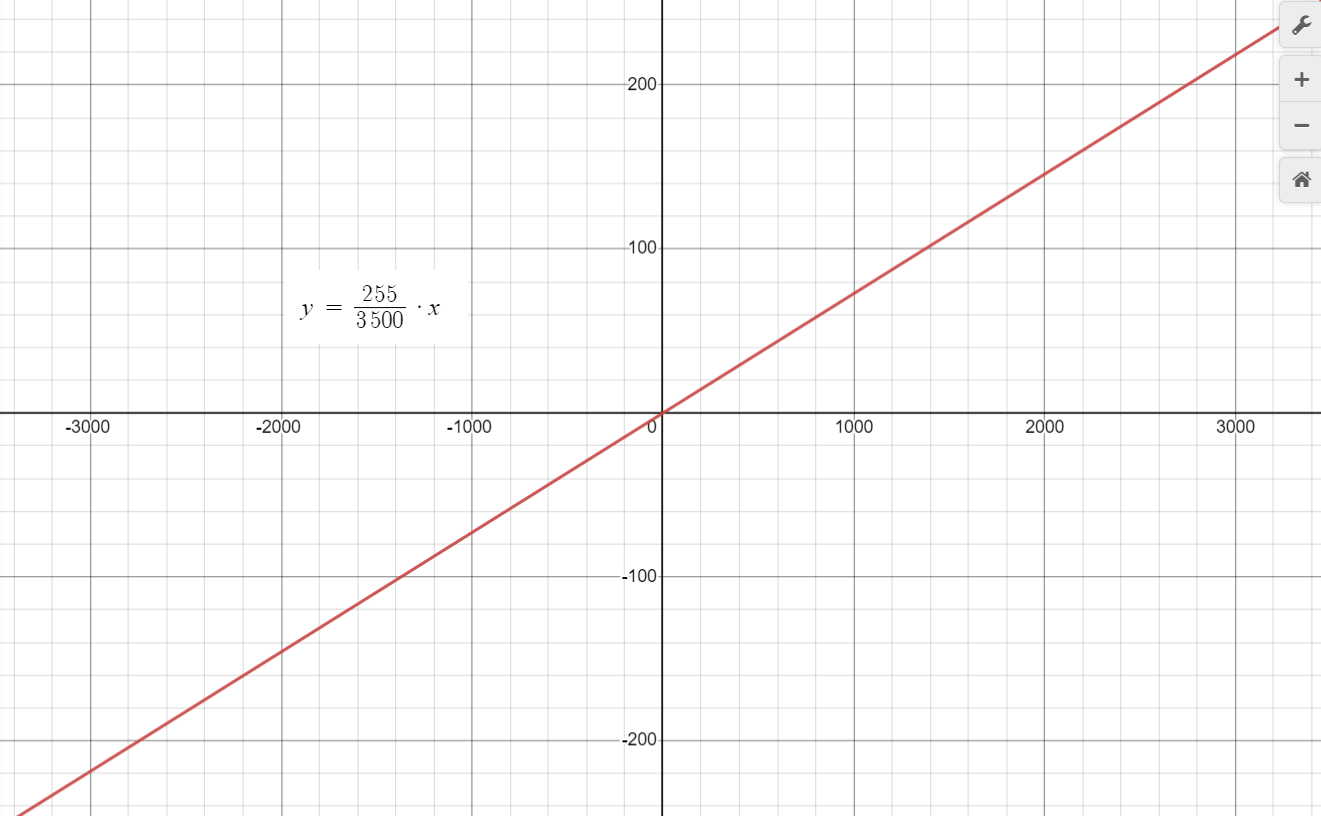
\includegraphics[width=\textwidth]{pictures/control/Linearization.png}
   \label{linerizationgraph}
\end{center}
\caption{PWM to angular speed, linearization}
\end{figure}

This linearity ensures when the PWM is 0 the angular speed is 0, and that the change in PWM is symmetrical for positive and negative values.